In this section we need to astablish some new properties for the class $\phi$. Much like in \autoref{sec:lQuasi}, the class need to have these proporties to be relevant for solving the weak $k$-linkage problem.\\ 
For a integer $c$, the class denoted $D(c)$ is a digraph $D$ where first there is added as many parallel arcs to arcs that already exists in $D$ then blow-up $b$ vertices where $0\leq b\leq c$, the digraph that is blown up has to have a size $\leq c$. 

\begin{definition}~\cite{bangJGT85}
    We say that a class of digraphs $\phi$ is Bombproof is there exsists a polynomial algorithm $\mathcal{A}_{\phi}$ to find a totally $\phi$-decomposition of every totally $\phi$-decomposable digraph and, for every integer $c$, there exists a polynomial algorithm  $\mathcal{B}_{\phi}$ to decide the weak $k$-linkage problem for the class
    \begin{equation}
        \phi(c):=\bigcup_{D\in \phi}D(c) 
    \end{equation}
    \label{def:bombproof}
\end{definition}
The clean houses $(D,\Pi)$ actually have an important part, namely the part that we do not need them for linking any of the piars of $\Pi$ in $D$.
\begin{lemma}~\cite{bangJGT85}
    Let $D$ be a digraph, $\Pi$ a list of $k$ terminal pairs and $H\subset D$ a clean house with respect to $\Pi$. Let $D'$ be the contraction of $H$ into a single vertex $h$. Then $D$ has a waek $\Pi$-linkage if and only if $D'$ has a weak $\Pi$-linkage.  
    \label{lemma:cleanhouse}
\end{lemma}
\begin{proof}
    \textcolor{red}{Maybe prove}
\end{proof}
The external pairs do not need the same amount of vertices and arcs inside a house as maybe the internal pairs. It turns out that in \cite{bangJGT77} we bound the number of vertices for the external paths. The lemma below is a reformulation of the lemma from \cite{bangJGT77}. 
\begin{lemma}
    Let $D=S[H_1,\dots H_s]$ be a decomposable digraph, let $\Pi'$ be a list of $h$ terminal pair and let $F$ be a set of arcs in $D$ satisfying that $d^-_F(v),d^+_F(v) \leq r$ for all $v \in V(D)$.
    If $(D\backslash F,\Pi')$ has a weak linkage, then it has a weak linkage $P_1,\dots , P_h$ such that, we have $|V\left( \bigcup_{i\in \mathcal{E}} P_i\cap H_j \right)|\leq 2h(h+r)$, for every $j\in [1,\dots,s]$, where $\mathcal{E}$ denotes the set of indeces $i$ for wich $P_i$ is external.
    \textcolor{red}{omformulere}
    \label{lemma:external}
\end{lemma}
\begin{proof}
    \textcolor{red}{blablabalbalabal}
\end{proof}

As shortly explain we sometimes have to control the set of arcs already used $F$ but as we remove these arcs from the digraph it may longer belong to the class it did before. we therefore need to make sure the removing some arcs from a digraph do not affect that we have an algorithm for the weak linkage if we had one without removing the arcs.
\begin{lemma}
    Let $\mathcal{C}$ be a class of digraphs for which there exists an algorithm $\mathcal{A}$ to decide the weak k-linkage problem, whose running time is bounded by $f(n,k)$. Let $D=(V,A)$ be a digraph, $\Pi$ a list of $k$ pairs of terminals and $F\subseteq V\times V$ such that $D':= (V,A\cup F)$ is a member of $\mathcal{C}$. There exists an algorithm  $\mathcal{A}^-$, whose running time is bounded by $f(n,k+|F|)$, to decide whether $D$ has a weak $\Pi$-linkage.
    \label{lemma:deletarcs}
\end{lemma}
\begin{proof}
    \textcolor{red}{blabalbalalabalba}
\end{proof}
Now we are going to state the theorem that is used for the existens of the of our main algorithm in this section. This result is found by ... in .... .
\begin{thm}
    Let $\phi$ be a bombproof class of digraph. There is a polynomial algorithm $\mathcal{M}$ that takes as input a 5tuple $[D,k,k',\Pi,F]$ where $D$ is a totally $\phi$-decomposable digraph, $k,k'$ are natural numbers with $k'\leq k$,$\Pi$ is a list of $k'$ terminal pairs and $F\subseteq A(D)$ is a set of arcs satiesfying 
    \begin{equation}
        d_F^-(v),d_F^+(v)\leq k-k' \text{ for alle } v\in V(D)
    \end{equation}
    \begin{equation*}
        |F|\leq (k-k')2k
    \end{equation*}
    and decides wheter $D\backslash F$ contains a weak $\Pi$-linkage.
    \label{thm:mainalgo}
\end{thm}
   
To proof \autoref{thm:mainalgo} we first state the algorithm $\mathcal{M}$ then we prove that it works, and last that the time for the algorithm is polynomial. Since the existens of the algorithm lyes in the proof that it works and it is polynomial we will first state it explain it come with an example of the choiches that it makes and then we will prove that is indeed the alforithm mensioned in \autoref{thm:mainalgo}.
\begin{algorithm}   
    \algio{
        Digraph $D$, two natural numbers $k$ and $k'$ where $k'\leq k$, a list of $k'$ terminal pairs $\Pi$, A set of arcs $F\subseteq A(D)$ satiesfying:
        \begin{align*}
            d^-_F(v),d^+_F(v)&\leq k-k' \ \forall v\in V(D)\\
            |F|&\leq (k-k')2k
        \end{align*}
    }{
        Either "No weak-linkage exists" or "there exists a weak-linkage in $(D,\Pi)$ with arc set $F$."
    }
    \begin{algorithmic}[1]
        \IF{$\Pi=\emptyset$}
            \STATE output that a solution exists and return
        \ENDIF
        \STATE Run $\mathcal{A}_{\phi}$ to find a total $\phi$-decomposition of $D=S[H_1,\dots,H_s]$.
        \IF{this decomposition is trivial that is $D=S$}    
            \STATE $D\in \phi\subset \phi(1)$, so run $\mathcal{B}^-_{\phi}$ on $(D\backslash F,\Pi)$ to decide the problem and return.
        \ENDIF
        \STATE Find among $H_1,\dots, H_s$ those houses $K_1,\dots , K_l$ that contain at least one terminal. 
        Let $D'$ be obtaint by contracting all the clean houses. 
        Let $F'$ be the set of arcs obtaint from $F$ after the contraction.
        \STATE Let $\Pi^e\subset \Pi$ $(\Pi^i\subset \Pi)$ be the list of external (internal) pairs $(s_q,t_q)\in \Pi$.
        \FOR{every partion of $\Pi^i=\Pi_1\cup\Pi_2$ look for external paths linking the pairs in $\Pi^e\cup \Pi_1$ and internal pairs in $\Pi_2$}
            \IF{$\Pi ^e\cup \Pi _1=\emptyset$, then for $i=1,\dots ,l$:} \label{state:6a}
                \STATE run $\mathcal{M}$ recursively on input $[K_i, k, k'_i,\Pi \cap K_i, F\cap A(K_i)]$, where $\Pi \cap K_i$ denotes the list of terminal pairs that lie inside $K_i$ and $k'_i$ is the number of those pairs.
            \ENDIF
            \IF{$\Pi ^e \cup \Pi _1\neq \emptyset $} \label{state:6b}
                \STATE let $k_i'$ be the number of pairs in $\Pi _2\cap K_i$
                \FOR{each possible choice of $l$ vertex sets $W_i\subseteq V(K_i)$,$i=1,\dots,l$ of size $\min \lbrace |V(K_i)|,2(k'-k'_i)(k-k')\rbrace$ and arc sets $F_i\subseteq A(K_i\left< W_i\right>)\backslash F$, $i=1,\dots ,l$ with $F_i$ satisfying 
                \begin{align}
                    d^-_{F_i\cup(F\cap A(K_i))}(v),&d^+_{F_i\cup(F\cap A(K_i))}(v)\leq k'-k'_i.\\
                    |F_i|\leq &2(k'-k'_i)(k-k')
                \end{align}
                }
                    \FOR{every $K_i$}
                        \STATE remove all the vertices of $V(K_i)\backslash W_i$ and then all remaining arcs except those in $F_i$.
                    \ENDFOR
                    \STATE Define $D''$ to be the digraph obtaint from $D'$ with this procedure.
                    \STATE Run $B_{\phi}^-$ on $(D''\backslash F',\Pi^e\cup\Pi_1)$.
                    \FOR{$i=1,\dots,l$}
                        \STATE run $\mathcal{M}$ recursively on input $[K_i,k,k'_i,\Pi_2\cap K_i,F_i\cup(F\cap A(K_i))]$.
                    \ENDFOR 
                \ENDFOR
            \ENDIF
            \IF{the if statement in \autoref{state:6a} all intances examined are linked $\OR$ at  the if statement in \autoref{state:6b} there is a choice of $W_i,F_i,i=1,\dots,l$ such that all instances examined are linked} 
                \STATE output that a weak linkage exists and return.
            \ENDIF
        \ENDFOR 
        \IF{all choices of $\Pi_1,\Pi_2$ have been consideredwithout verifying the existens of any weak linkage}
            \STATE output that no weak linkage exists.
        \ENDIF
    \end{algorithmic}
    \caption{The main algorithm $\mathcal{M}$}
    \label{alg:weakphi}
\end{algorithm}


 

    First we deskribe wiht words what the input and output of the algorithm is. 
    The output is already written in words and is very undestandeble. \\
    The input can be elaborated somewhat more, first $\mathcal{M}$ is polynomial but also recursively defined. 
    It decides whether $(D,\Pi)$  has a weak-linkage on overall $k$ terminals. 
    Since the algorithm is recursive it does not find all the solutions in one go therfore we define $k'$ as the number of terminals that we still need to find a weak linkage for, and $F$ is a part of the solution of at most $k-k'$ already found weak-linkages of $D$, $\Pi$ is the set of terminals that we what to find the weak linkage for. \\
    So you can in the begining have $F=\emptyset$ and $k=k'$. This will help on the undestaniding of the algorithm.    
 
     
    Step 1: "$\Pi=\emptyset$" makes sure that if we call the algorithm $\mathcal{M}$ with no pairs then there exists the solution with zero acrs to solve the weak-linkage problem. \\

    Step 2: Recall that the digraph is totally $\phi$-decomposable and $\phi$ is bomproof and from \autoref{def:bombproof} we know tha the digraph has a algortihm $\mathcal{A}_{\phi}$ that gives the $\phi$-decomposition of the digraph. \\

    Step 3-5: From \autoref{def:bombproof} we know that $\mathcal{B}_{\phi}$ decides a weak-linkage for $D\in \phi$, since we cant guarentee that $D\backslash F \in \phi$ we use \autoref{lemma:deletarcs} that tells us that $\mathcal{B}_{\phi}^-$ can decide a weak-linkage in $D\backslash F=(V,A\backslash F)$ if $D' \in phi$ $D'=(V,(A\backslash F)\cup F)=(V,A)=D\in \phi$. \\

    Step 6: Here we find all the non-clean houses from $H_1,..,H_s$ and contract all the clean houses w.r.t. $\Pi$ we make a new nummeration of all the non-clean houses $K_1,\dots ,K_l$ of $D$ w.r.t. $\Pi$
    Since by \autoref{lemma:cleanhouse} we know that contracting one clean house in $D$ if it has a linkage so does our new digraph, then use this lemma agian and agian until there is no more clean houses.
    This is our new digraph $D'$ with non-clean houses $K_1,\dots,K_l$ and if we find a weak linkage w.r.t. $\Pi$ in $D'$ we know that $D$ has a weak linkage from continueing using \autoref{lemma:cleanhouse}.
    We also let $F'=F\cap A'$ where $A'$ is the arcset of $D'$.\\

    Step 7: Recall an internal pair is where both vertices is in the same house and an external pair is where the vertices is two different houses. 

    Step 8: This for loop is looking for two different cinds of path between internal pairs since the path for an internal pair can be an internal path (fully cept in the house) or an external path going out of and later in the house. 
    For simplyfication look at \autoref{fig:internalpair}
    \begin{figure}
        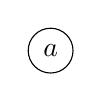
\begin{tikzpicture}[main/.style ={draw,circle}]
            \node[main](a) {$a$};
        \end{tikzpicture}
        \label{fig:internalpair}
    \end{figure}

    Step 9-11: if $\Pi^e\cup \Pi_1=\emptyset$ , either we have already found all external path in this partition or there was none. 
    Either way all terminal pairs left is internal so and $\Pi =\Pi_2$. So we are only interesten in finding the internal path of the internal pairs, which is why we can call $\mathcal{M}$ on each house for itself.
    Each $K_i$ could be a big graph in itself that is decomposable with at least some house $H_i$ where $|H_i|\geq 2$, if this is not the case the algorithm returns after step 3: and continue with the next. 
    If $\mathcal{M}$ has already found some external paths $F$ might not be empty  and may use some arcs inside $K_i$ therefore $F\cap A(K_i)$. $\Pi \cap K_i$ is becouse we are not interested in the terminal pairs that are not a part of the graph we are looking at (pairs inside $K_j$ where $j\neq i$).

    Step 12: Looking for external paths in a big graph is a bit more deficualt since we do not know which arcs and vertices not to use.
    
    Step 13-14: First we find all the pairs that is internal pairs, we want to link as internal paths, the number of these is $k'_i$ for each $i=1,\dots l$. Then we choose a very specifik size of vertex sets $W_i$ and loop over every choiche of these. These vertex set induces a subdigraph, where we make a possible arc set where inside not containg what is inside $F$ we call these $F_i$ we make these set as big as possible linkage need for the rest of the terminal pairs (those we want to find external paths of$\Pi^e\cup \Pi_1$) the number of those is $k'-k'_i$ since every pair mabey has to go through the house we are looking at.
    
    Step 15-19: For each house we remove all vertices not in the vertex set $W_i$ after removing these vertices we remove all remaining arcs except those arcs in $F_i$.
    This is defined in the algorithm as $D''$. We can show that $D''\in \phi(2k^2)$. First we know that since $D$ is totally decomposable $S\in \phi$ and from \autoref{def:bombproof} and the definition on $D(c)$ we can take $S$ add as many parralelle arcs as we want we only need to blow up $l$ vertices those houses of $D$ that are not clean we know that there is $k'$ terminal pairs and that $k'\leq k$ meaning $l\leq 2k$ these $l$ vertices needs to be blown up and from lemma \autoref{lemma:external} lets say that we want to find $k''\leq k'$ external paths in $D$ ($|\Pi^e \cup \Pi_1|=k''$) then we are only looking at $k''$ terminals meaning in every blow up we need at most $2k''(k''+(k-k'))$ since $k''\leq k'$ we have $2k''(k''+(k-k'))\leq 2k''k$ vertices in $W_i$ and $2kk''\leq 2kk'\leq 2k^2$ which is the biggest number we will need to blow up the $l$ vertices meaning $c=2k^2$ so $D''\in \phi (2k^2)$.

    Step 20-24: We need to make sure that the tuple $[K_i,k,k'_i,\Pi_2 \cap K_i,F_i\cup(F\cap A(K_i))]$ upholds every condition for every choice of that tuple. 
    Since we are not focusing on loops we know that the max number of arcs is bounded by the max number of vertices $|F_i|\leq 2kk''$ the rest of the terminals is the number of internal pairs which we in the algorithm denote $k'_i$. we know that $k'_i\leq k'-k''$ meaning $k''\leq k'-k'_i$.
    we start calculating the to demands of $F$ in the tuple.
    Note that $d_{(F\cap A(K_i))}(v)=d_{F}(v), \ \forall v\in V(K_i)$ and we also know $d_{F_i}(v)\leq k''$ so
    \begin{align}
        d^+_{F\cup F_i},d^-_{F\cup F_i}\leq k-k' + k'' = k-(k'-k'')\leq k- k'_i \\
        |(F \cap A(K_i))\cup F_i|\leq |F|+|F_i|\leq 2k(k-k') +2kk''\\
        \leq 2k(k-\textcolor{blue}{k'})+2k(\textcolor{blue}{k'}-k'_i)=2k(k-k'_i).
    \end{align}
    Clearly the tuple for $F$ holds forall its conditions.

\textcolor{red}{Example of algorithm $mathcal{M}$}
\begin{proof}
    We have now proved and explained each step in the algorithm, that it does what we think. 
    Now we need to check whether given your favorite digraph, that upholds the conditions, the algorithm gives the right result.
    If the digraph do not terminate before examine list $\Pi^e\cap \Pi_1$ of $k''$ terminal pairs if $k''=0$ we enter step 9 and $F_i=\emptyset, \text{ for } i=1,\dots l$, and by the induction hypothesis we can assume that if there exists a weak linkage in each $K_i$ the algorithm would find it. 
    Now if this is not the case and $k''>0$ step 12 is then entered and we construct $D''$ which we have described belong to $\phi(2k^2)$ and then as descirbed before we can use $B_\phi^-$ which is correct by \autoref{def:bombproof}, so the algorithm will find a weak $\Pi''$-linkage if it exists in $D''\backslash F'$. 
    After all this there is made a recursiv call on each $K_i$ finding $k'_i$ weak linkages and by the above proof we know it works. 
    So since $B_\phi^-$ correctly finds the weak linkage inside $D''\backslash F'$ using only arcs from $F_i$ $\forall i\in[l]$, then each $K_i$ is recursively called from $D''$ we can easily come back to $D'$ since we find the weak $k'_i$-linkage inside each $K_i$ which is not using any of the arcs from $F_i$ we know that together these stil form the seperated weak linkages.
    By \autoref{lemma:deletarcs} we know that we can find a weak linkage in $D\backslash F$ if we can find it in $D''\backslash F'$ which just proved we can. given a perfekt weak $\Pi$-linkage.
 \textcolor{red}{Polytime...}
\end{proof}

\subsection{$k$-linkage problem for quasi-transitive digraphs}
We have already establish in \autoref{sec:quasi} that quasi-transitive digraphs are totally $\phi_1$-decomposable.
It turns out that we just have to prove that $\phi_1$ is bombproof, for that we need the two polynomial algorithms $\mathcal{A}_{\phi_1}$ and $\mathcal{B}_{\phi_1}$. Recall that $\phi_1$ is bulid up by semicomplete and acyclic digraphs so we need to establish some theorems for the weak $k$-linkage problem on semicomplete and acyclic digraphs.
\begin{thm}
    The weak $k$-linkage problem is polynomial solvable for every fixed $k$ when the input ia an acyclic digraph.
\end{thm}
\begin{thm}
    The weak $k$-linkage problem polynomial for every fixed $k$, when we consider digraphs that are obtained from a semicomplete digraph by replacing some arcs with multiple copies of those arcs and adding any number of loops.
\end{thm}

Since the bombproof class alows the digraph to no longer be a part of that class we need to consider that an acyclic digraph can get a cycle when blowing up a vertex. 
\begin{thm}
    For every natural number $p$ the weak $k$-linkage problem is polynomial for every fixed $k$, when we consider digraphs with most $p$ directed cycles.
\end{thm}
% This is a direct consequence of 
%\begin{thm}
%    For every natural number $\theta$ the weak $k$-linkage problem is polynomial for every fixed $k$, when we consider digraphs with cutwidth at most $\theta$.
%\end{thm}

Now we can prove that $\phi_1$ is bombproof and therefore that quasi-transitive digraphs have a polynomial solution for the weak $k$-linkage problem, when $k$ is fixed.

\begin{thm}
    The class $\phi_1$ is bombproof.
\end{thm}
\begin{proof}
    \textcolor{red}{blablabalbalablab}
\end{proof}

